


\chapter{SCR for Search-Encounter Data}
\markboth{Chapter 16}{}
\label{chapt.searchencounter}

\vspace{0.3cm}


\section{Royle and Young model}

\section{MHB data}

\section{Mountain Lion Analysis}

\section{Fisher crap}

\section{Capricaillie crap}

We provide an example of the Poisson model from 
 \citet{mollet_etal:2012}, who obtained a population
size estimate  of a large forest grouse species known as the
capracaillie in a region of Switzerland. 

In this study, 
8 forest stands  that represent all available habitat of the
species were sampled. Each of the stands was divided into a number of
fragments, each of 
sufficient size to sample in a meaningful way, creating 39 patches of around
30-70 ha each. For modeling we further divided each patch roughly in half to
create 78 spatial sample units -- so scat samples could be associated to one of
the 78 sub-units. This was done mostly for the purpose of creating spatial
replicates. If the 39 larger units were used there were relatively little
realized spatial replicates. 
We did not use finer scale things because searching was rather opportunistic
and haphazard within a unit. Observers searched out what they thought was
good opportunity to find scats but we don't know the whole extnet of
sampling..........

Importantly, the sample units are actually large forest
patches on the order of tens of ha each, but variable in size. Data
were {\it not} collected by coordinates of observations but rather
just recorded to the specific patch in which the observation was
encountered. To accomodate this we defined ${\bf s}_{i}$ to be a
discrete
random variable taking on values...........................

Forest patches were searched for scat which was
situation in which discrete patches of habitat are searched using some
method and it might be convenient (or occur inadvertently) to
associate samples to the patch level instead of recording observation
locations. In this case we might use a model $s[i] \sim dcat(probs[])$
where $probs[]$ are the probabilities that an individual inhabits a
particular patch.

samples are spatial encounter frequencies of scat essentially and so
it makes sense to think of them as Poisson or other.
In fact there's a bit of opportunistic thinning going on but we'll view
this as random thinning and still asert that the encounter frequencies
are Poisson with constant $\lambda_{0}$ and individual intensity that
depends on distance according to the bivariate normal model. 



\begin{figure}
\centering
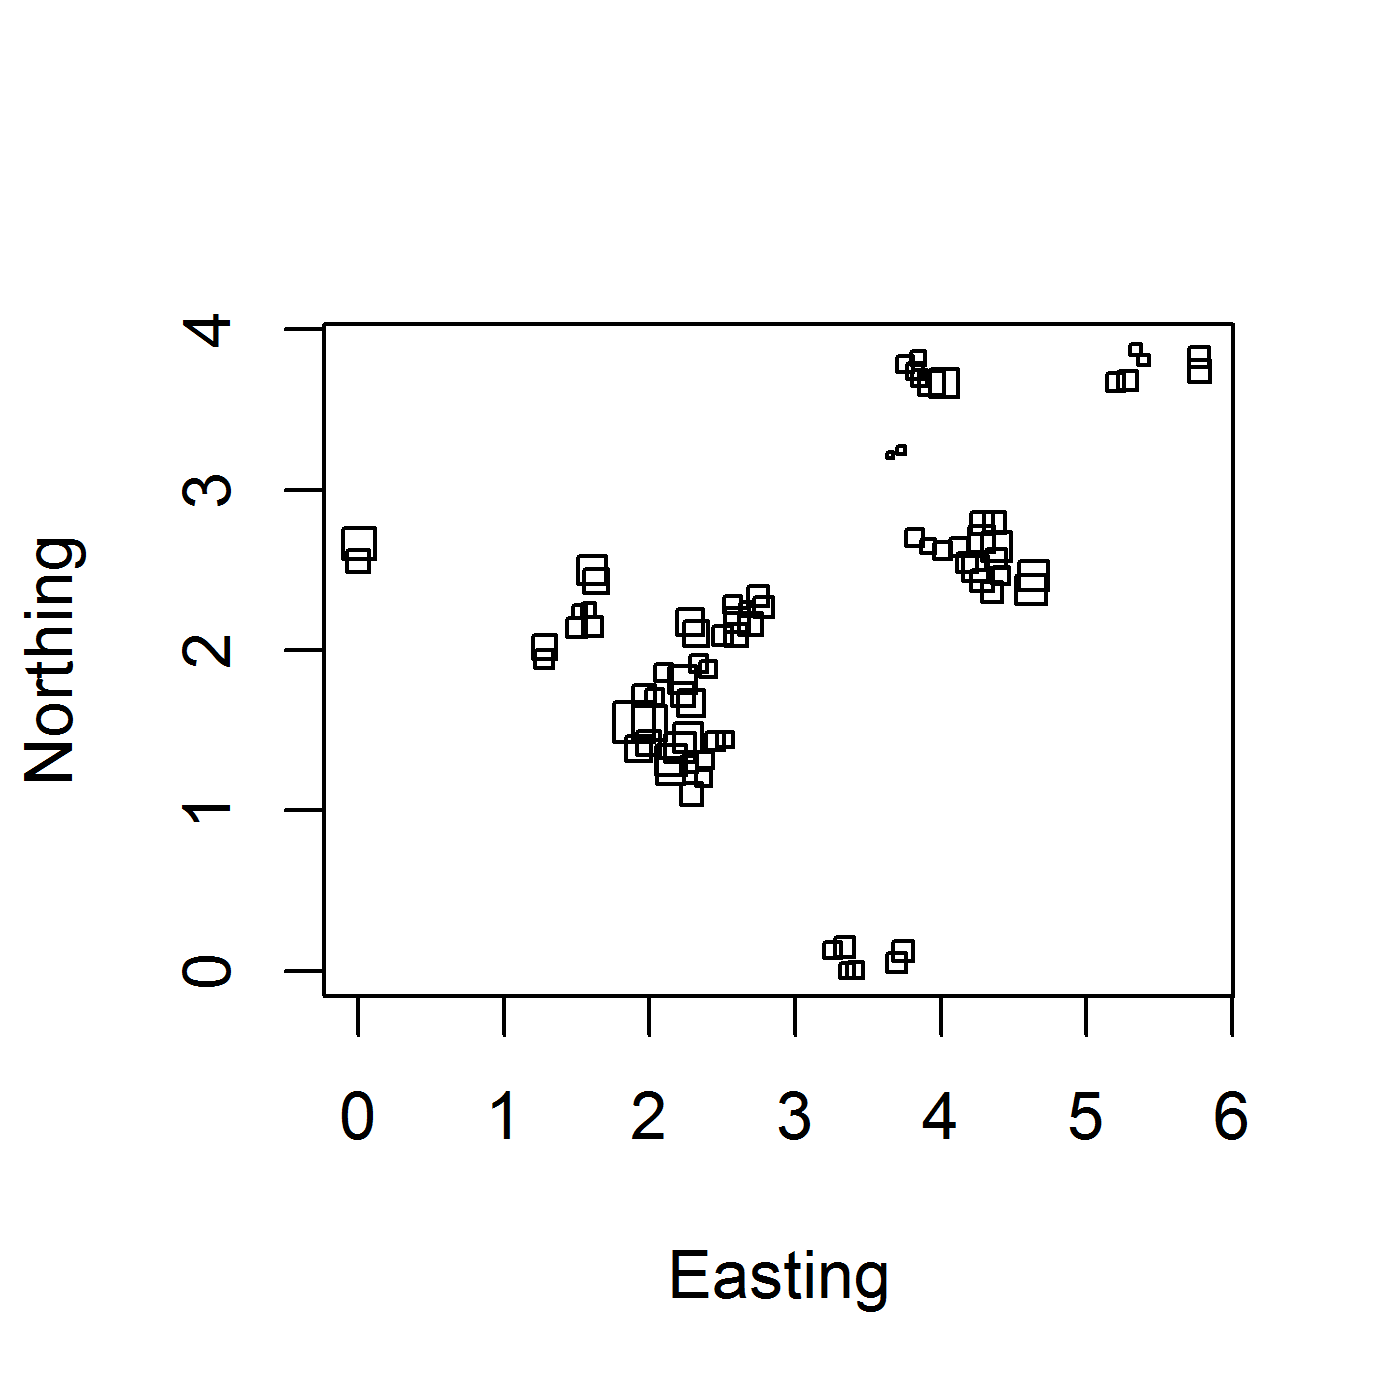
\includegraphics[width=3.5in,height=3.5in]{Ch5/figs/Cap-fragments.png}
\label{poisson-mn.fig.capfrags}
\caption{Relative size and position of 78 forest fragments sampled for
  capricaillie crap.}
\end{figure}


Each of the 44 units
could be sampled by one person in
one day's work (6-8 hours). Within each unit, we focused our search
for droppings on the areas below roosting trees and feeding trees,
respectively, in hiding sites, along internal forest edges, around
root plates and on tree stumps (cf. Jacob et al. 2010). These habitat
elements are the ones preferred by the birds in winter at a small
spatial scale (Bollmann et al. 2005; Mollet unpublished data).
Five spatial units ($I_a$, $S_a$, $S_b$, $H_a$, $T_a$, Table 2) could
not be sampled because of time constraints (too few days with
favorable weather conditions), resulting in 39 units sampled. For the
same reason, three units $(I_b, W_1, W_a)$ were sampled only
once. Access to the area B (Fig. 2) is possible only in late
spring. In 2009, sampling started on 20 April, and the three units in
area B could be sampled only once (rapid snow melting towards the end
of April precluded repetition of sampling here). All other units were
sampled twice.




\subsection{model}

activity centers were uniformly distributed to each of the 78
fragments in proportion to area of the forest patch within which each
fragment was located.


We parameterized activity centers by a discrete state-space with elements
corresponding to the 8 larger fragments. Moreover, home ranges were allocated
to each fragment in  proportion to area. i.e., we assume
define $\lambda_{frag} = A_{frag} \lambda_{0}$, and then:
\[
 N_{frag} \sim Poisson( A_{frag} \lambda_{0} )
\]
This assumption implies the following prior distribution on ${\bf s}_{i}$ (Chapt.
XYZ; Converse and Royle 2012):
\[
{\bf s}_{i} \sim  \mbox{Categorical}(  \pi_{frag} ) 
\]
with
\[ 
 \pi_{frag} = \frac{ \lambda_{frag} }{\sum_{frag} \lambda_{frag}}
\]


Observation model:  

Each of the 78 fragments is its own sample unit which we index to the
center point of the fragment. No finer scale information is made about
the observation locations. 
Let $y_{ij}$ be  the number of times individual $i$ encountered in stand $j$.
Note these are not unique droppings but rather unique clusters of
droppings because a grouse roosting in a tree might leave a number of
droppings and only one of them was sampled\footnote{perhaps this is
  too optimistic of an assessment?}. 






